\section{Make OTB in QGIS Great Again!}

\begin{frame}
\frametitle{2009: OTB-QGIS plugin (Archéologie)}
\begin{minipage}[t][6cm][t]{\textwidth}
\begin{center}
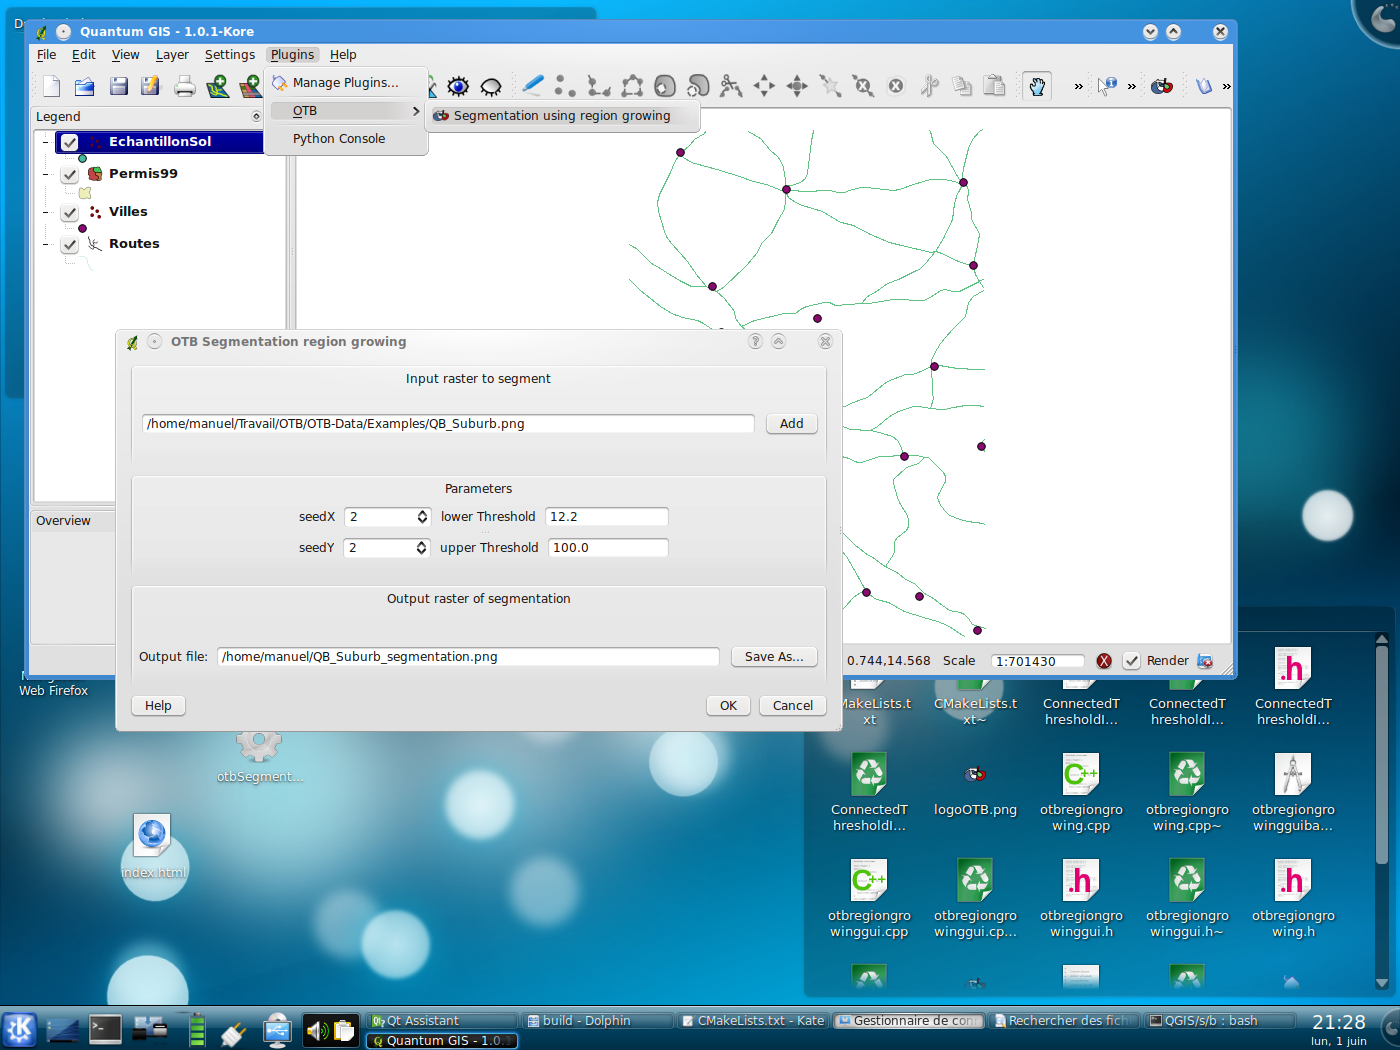
\includegraphics[width=0.7\textwidth]{images/otb-qgis-2009.png}
\end{center}
\end{minipage}
\end{frame}

\begin{frame}
\frametitle{2012-2017: OTB-QGIS disponible via le module processing}
\begin{minipage}[t][6cm][t]{\textwidth}
\begin{center}
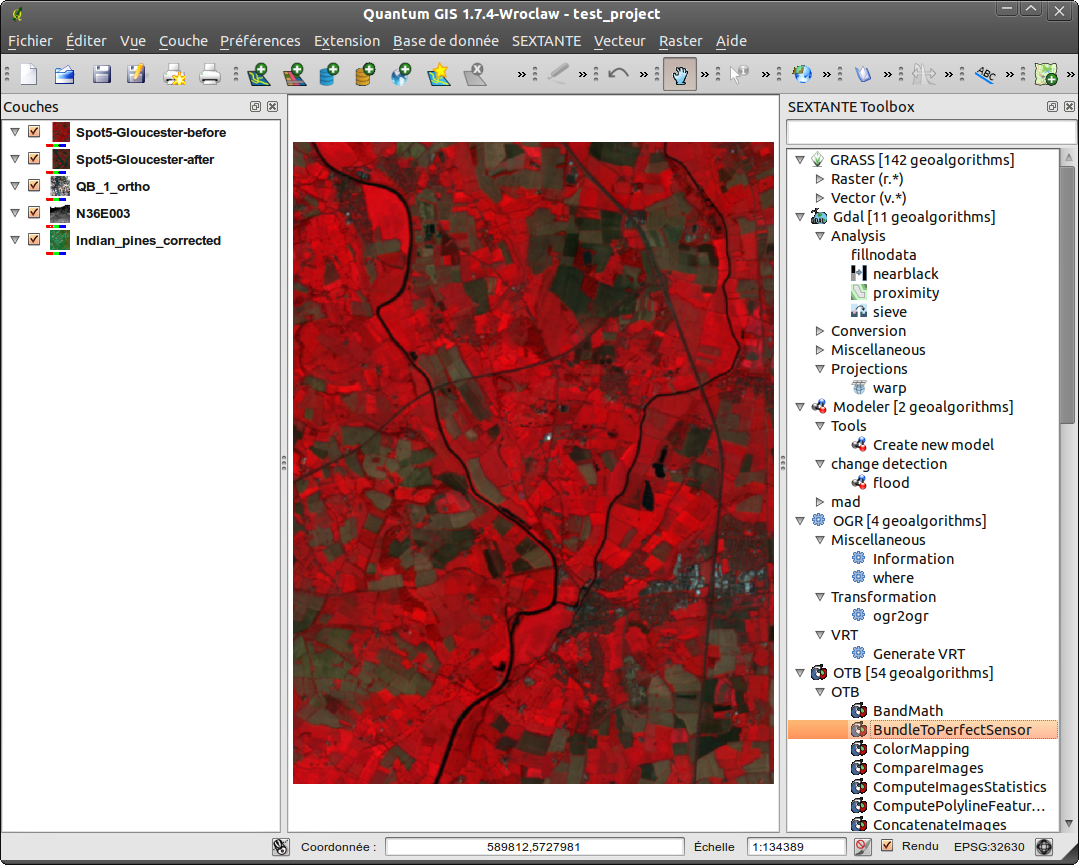
\includegraphics[width=0.7\textwidth]{images/otb_qgis.png}
\end{center}
\end{minipage}
\end{frame}

\begin{frame}
\frametitle{Accès OTB dans QGIS: A powerful wedding}
\begin{itemize}
\item Facilite l'accès à l'OTB (QGIS is mainstream)
\item Profite de l'interface et des fonctionnalités de QGIS (OTB GUI...)
\item Intégration dans le module ``processing'' de QGIS (bactch, Python...)
\item Collaboration très positive avec la communauté QGIS
\item Support des développeurs QGIS
\item OSGeo \textit{power}
\item \href{https://www.youtube.com/watch?v=ufSQ2SgSIV4}{Démo}: \url{https://www.youtube.com/watch?v=ufSQ2SgSIV4}
\end{itemize}
\end{frame}

\begin{frame}
\frametitle{Mais aussi des problèmes...}
\begin{itemize}
\item ``Comment on installe la dernière version de l'OTB dans QGIS?''
\item ``Quelles versions de l'OTB fonctionnent avec quelles versions de QGIS?''
\item ``Pourquoi l'application de segmentation OTB n'apparaît pas dans le menu QGIS?''
\item ``Pourquoi les applications OTB n'ont pas le même nom dans QGIS?''
\item ``J'abandonne OTB dans QGIS, rien ne fonctionne...''
\item \alert{STOP!}
\item 2018: on va améliorer tout ça
%\item Maintenance, Maintenance, Maintenance...
%\item Each version of otb needs to update list of descriptor files
%\item XML files which are hard to maintain.
%\item requires to update a blacklist and whitelist documents to list app that cannot be included and can be included
%\item needs manual update of these xml + followup on pull request
%\item works only with limited version of OTB (Not last release, mostly behind 3-4 releases)
%\item Nobody want to work on it from otb and qgis side. maintained by CS team
%\item Some applications were grouped, depending on their parameters : BinaryMorphologicalOperation (Closing, Dilate, Erode, Opening)
%\item Add new parameter in ParameterMultipleExternalInput processing, to use it in FusionOfClassifications
\end{itemize}

\end{frame}

\begin{frame}
  \frametitle{2018: OTB-QGIS plugin - L'âge de la maturité}
  \begin{itemize}
    %\item Easy maintenance for both OTB team and QGIS team
  \item Keep It Simple
  \item Faciliter la maintenance des versions OTB (pour les équipes OTB et QGIS)
    %\item Descriptors are generated, distributed and maintained by OTB
  \item Binaires OTB: Support QGIS ``out of the box''
  \item Toutes les applications OTB sont disponibles dans QGIS (même nom, même documentation...)  
    %\item Out of box support for qgis via binary packages
    %\item Applications are not grouped.
    %\item Development took a turn due to some *non-technical*/politic issues in
    %qgis and otb
  \item \alert{Version bêta} disponible sous la forme d'un plugin
  \item Plugin sera prochainement ajouter aux sources de QGIS
    %\item Will be added back to QGIS processing core later (Thanks to QGIS team)
    %\item Support for remote modules
    %\item OTB processing provider knows to recreate descriptor file for apps (if not found)
    %\item \alert{Version beta} disponible sous la forme d'un plugin
    % First version is distributed a plugin
  \item
    Code source du plugin: \url{https://gitlab.orfeo-toolbox.org/orfeotoolbox/qgis-otb-plugin}
  \item Compatible de QGIS 3.2
  \item Merci aux équipes QGIS!
  \end{itemize}
\end{frame}

\begin{frame}
\frametitle{Configuration provider OTB dans QGIS}
\begin{center}
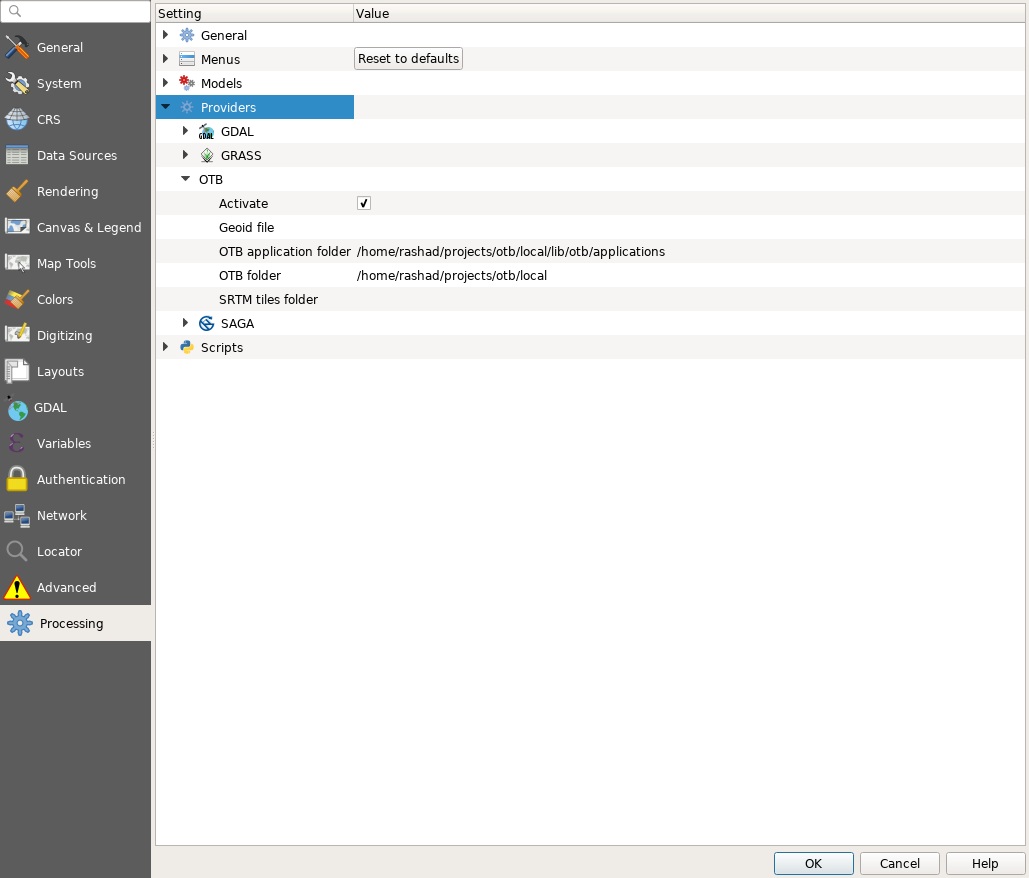
\includegraphics[width=0.8\textwidth]{images/qgis_otb_provider_config.png}
\end{center} 
\end{frame}

\begin{frame}
\frametitle{Interface de l'application \textit{Smoothing}}
\begin{center}
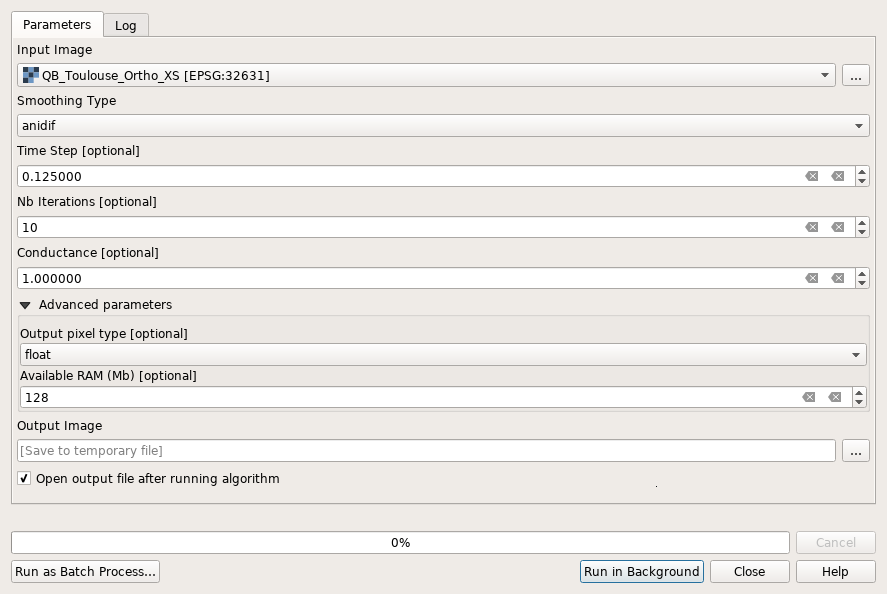
\includegraphics[width=0.8\textwidth]{images/qgis_smoothing.png}
\end{center} 
\end{frame}

\begin{frame}
\frametitle{Interface de l'application \textit{TrainImagesClassifier}}
\begin{center}
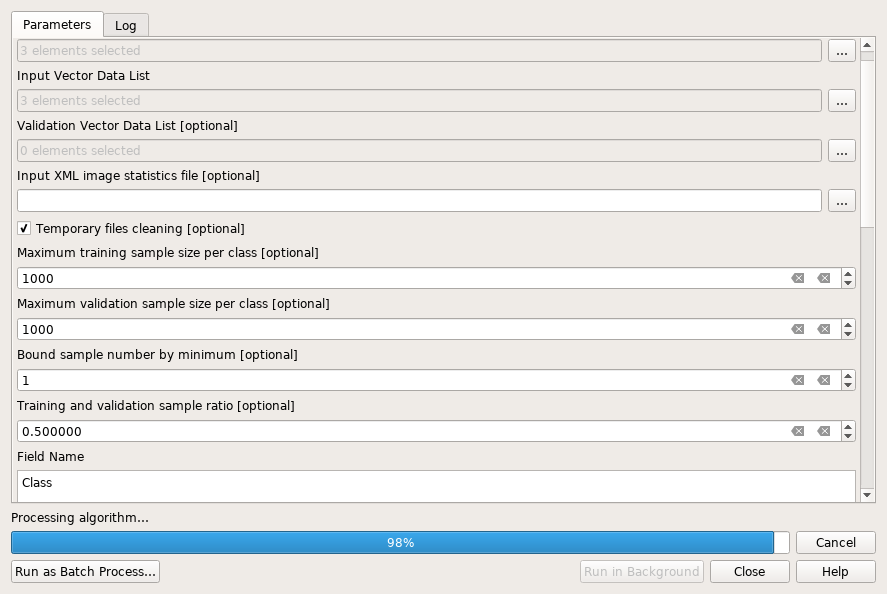
\includegraphics[width=0.8\textwidth]{images/qgis_train_classif.png}
\end{center} 
\end{frame}
